% !TeX program = pdflatex
% !TeX encoding = UTF-8
% !TeX spellcheck = es_ES
% (Sin bibtex/biber: la bibliografía es un entorno thebibliography en referencias/referencias.tex)
\documentclass[10pt,a4paper]{article}
\usepackage[utf8]{inputenc}
\usepackage[spanish,es-nodecimaldot]{babel}
\usepackage{textcomp}
\addto\captionsspanish{\renewcommand{\tablename}{Tabla}\renewcommand{\refname}{Referencias}\renewcommand{\figurename}{Figura}}
\usepackage{amsmath,amssymb,mathtools}
\usepackage{float}
\usepackage[protrusion=true,expansion=false]{microtype}
\usepackage[round,authoryear]{natbib}
\usepackage{water_like}              % estilo emulado de Water (MDPI), archivo water_like.sty
\usepackage{xurl}
\usepackage[hidelinks]{hyperref}
\setlength{\bibhang}{0.9cm}\setlength{\bibsep}{2pt}
\renewcommand{\bibfont}{\small}
\graphicspath{{figuras/}}
\newcommand{\Qs}{\mathrm{m^3/s}}
\newcommand{\pc}{\text{\thinspace\%}}  % porcentaje con espacio fino (evita "Incompatible glue units" con babel español)
\newcommand{\repo}{\url{https://github.com/Quioz/Prueba-collab}}

\begin{document}
\thispagestyle{firstpage}
\noindent\wlogo{figuras/logo_posgrado_recortado.png}\hfill{\footnotesize\color{wgrey}\begin{tabular}{r}Universidad Nacional de San Cristóbal de Huamanga\\Maestría en Hidráulica e Hidrología · Curso MIH-626\end{tabular}}\\[-2pt]
{\color{wgrey}\rule{\textwidth}{0.5pt}}\\[8pt]
\noindent{\large\bfseries Artículo}\\[10pt]
{\raggedright\fontsize{17}{20}\selectfont\bfseries Reparto de caudal en una bifurcación de canales rectangulares: formulación de energía, solución por Newton--Raphson y contraste con HEC-RAS 2D en cinco ángulos\par}
\vspace{10pt}
\noindent{\bfseries Brigmar Prado Taquire, Giomar Rubenney Quispe Ozaita y Luis Jhonatan Zamora Guillen}\\[5pt]
{\small Escuela de Posgrado, Universidad Nacional de San Cristóbal de Huamanga, Ayacucho, Perú (Grupo 7)\\
Correspondencia: \href{mailto:giomar.quispe.16@unsch.edu.pe}{giomar.quispe.16@unsch.edu.pe}}
\vspace{10pt}

\noindent\begin{wmeta}
\wsection{Datos del manuscrito}\\
Curso: Flujo en superficie libre (MIH-626).\\
Docente: MSc. Iván Arturo Ayala Bizarro.\\
Trabajo 01, estructura n.º 8: confluencia o bifurcación de canales.\\
Versión: final para entrega, noviembre de 2026.

\wsection{Cita sugerida}\\
Prado Taquire, B.; Quispe Ozaita, G.R.; Zamora Guillen, L.J. Reparto de caudal en una bifurcación de canales rectangulares. Trabajo 01, MIH-626, UNSCH, 2026.

\wsection{Aviso}\\
Documento académico con el aspecto de un artículo de Water; no ha sido publicado por MDPI.
\end{wmeta}\hfill
\begin{wabstract}
\wsection{Resumen:} Se estudia el reparto de un caudal de $12\,\Qs$ entre dos ramales rectangulares (3 m y 2 m de ancho) de un canal principal de 4 m, para ángulos de bifurcación de $30^\circ$, $45^\circ$, $60^\circ$, $90^\circ$ y $120^\circ$. Se resuelven por Newton--Raphson dos formulaciones unidimensionales: (I) flujo plano ideal con tapa rígida, que fija el reparto solo con la geometría, y (II) balance de energía por ramal con nivel común en la unión, pérdida local y fricción de Manning. La Formulación II da $Q_2/Q_0=0.4216$ con los datos nominales, independiente del ángulo, y es poco sensible a la pérdida local ($\varphi$ varía menos de $0.01$ al pasar $K$ de 0 a 2.4). Los resultados se contrastan con HEC-RAS 2D (ecuaciones SWE-EM, hidrograma de 0.5 a $12\,\Qs$ mantenido 7200 s, nivel fijo en las salidas, celda de 0.25 m) con balance de volumen $\leq0.009\pc$ en los cinco ángulos. El 2D da $\varphi=0.374$, $0.358$, $0.350$, $0.340$ y $0.313$: decrece con el ángulo, con una tendencia opuesta a la de la Formulación I (de $0.406$ a $0.785$) y sin la constancia de la II, que sobrestima $Q_2$ entre $+13$ y $+35\pc$. Ese 2D no es una referencia convergida: la fricción efectiva del modelo cae al refinar la malla ($n_\mathrm{eff}/n=0.93$, $0.86$ y $0.72$ para celdas de 0.50, 0.25 y 0.125 m en ramales rectos aislados) y $\varphi$ a 30° pasa de $0.389$ a $0.343$; una corrección lineal de $n$ no cumple la tolerancia de $\pm0.01$ m. Un conjunto exploratorio con SWE-ELM da $\varphi\approx0.41$ entre $30^\circ$ y $60^\circ$ y reduce la brecha con la II a $3\pc$, pero ese conjunto no pasó la verificación en ramales diagonales. La conclusión robusta es que la Formulación I queda contradicha a ángulos grandes y que ninguna formulación 1D reproduce la tendencia con $\theta$; el nivel exacto de $\varphi$ depende de la malla y de las ecuaciones del 2D. Se entregan datos y código para reproducir los resultados.
\wkeywords{bifurcación de canales; reparto de caudal; Newton--Raphson; energía específica; sensibilidad; HEC-RAS 2D; dependencia de malla}
\end{wabstract}
\vspace{6pt}{\color{wgrey}\rule{\textwidth}{0.5pt}}

\section{Introducción}
El reparto del caudal en una bifurcación de canales abiertos determina el dimensionamiento de canales de riego, derivaciones y obras de control. La literatura experimental y numérica muestra que la fracción derivada depende del ángulo, de la relación de anchos, del número de Froude y de las condiciones aguas abajo, y que las zonas de separación y recirculación junto a la esquina de la derivación modifican la sección efectiva de flujo \citep{ramamurthy1988,ramamurthy1990,hsu2002,momplot2017,ibrahim2022,gumgum2026}. Los modelos unidimensionales (1D) resuelven la unión mediante continuidad, igualdad de niveles y pérdidas locales, y son baratos y fáciles de integrar en redes \citep{chaudhry2008,chow1959}; los modelos bidimensionales (2D) capturan la redistribución lateral, pero dependen de la malla, de la rugosidad y de las condiciones de borde \citep{ghostine2012,ramamurthy2007}.

Para una bifurcación dada, el ingeniero necesita saber (i) qué formulación 1D reproduce el reparto con un error aceptable, (ii) de qué parámetros depende más ese reparto y (iii) si las diferencias frente a un modelo 2D son un defecto de la formulación o un efecto de configuraciones no equivalentes. Las comparaciones 1D--2D publicadas suelen reportar el acuerdo, pero no separan estas causas \citep{ghostine2012,gumgum2025}.

Este trabajo aborda tres objetivos para un caso sintético: (1) resolver por Newton--Raphson dos formulaciones del reparto y verificar el código; (2) cuantificar la sensibilidad del reparto a los parámetros y propagarla a una incertidumbre paramétrica; y (3) contrastar las dos formulaciones con simulaciones HEC-RAS 2D en cinco ángulos, verificando antes el modelo 2D contra el remanso 1D en ramales rectos aislados y examinando su dependencia de la malla y de las ecuaciones. El aporte no es un modelo nuevo, sino un procedimiento reproducible para decidir cuándo una formulación 1D de la unión es suficiente y cuándo no, junto con una lista explícita de lo que la comparación efectuada no permite concluir.

El artículo sigue el orden habitual de Water: marco teórico (Sección~\ref{sec:teoria}), materiales y métodos (Sección~\ref{sec:metodos}), resultados (Sección~\ref{sec:resultados}), discusión (Sección~\ref{sec:discusion}) y conclusiones (Sección~\ref{sec:conclusiones}).

\section{Marco teórico}\label{sec:teoria}
\subsection{Continuidad y condición de unión}
Para flujo permanente e incompresible, sin almacenamiento en el nodo, $Q_0=Q_1+Q_2$. Se denota la fracción derivada al ramal 2 por $\varphi=Q_2/Q_0$. El régimen local se caracteriza por el número de Froude $Fr=V/\sqrt{gD}$, con $D=A/T$; para una sección rectangular $D=y$. Se adopta $z_J$ como cota de solera común en la unión, y las dos ramas comparten en la sección de unión el nivel de superficie libre $H_J=z_J+y_J$, sin que ello implique igualdad de velocidades ni de cargas totales.

\subsection{Formulación I: flujo plano ideal con tapa rígida}\label{sec:f1}
Como cierre independiente de la energía y de la fricción, una bifurcación puede idealizarse como flujo plano, permanente, irrotacional y no viscoso, con superficie libre aproximada por una tapa rígida (límite de $Fr$ pequeño). Con el potencial complejo $w=\phi+i\psi$ y la geometría poligonal, el mapeo de Schwarz--Christoffel conduce a la solución de Milne-Thomson para paredes semiinfinitas \citep[\S 10.8]{milnethomson1962}; véase también \citet{batchelor1967} y \citet{gurevich1965}. Sean $\lambda=b_1/b_0$ y $\mu=b_2/b_0$ las relaciones de ancho, $u_i=U_i/U$ las velocidades lejanas adimensionales y $e=1-\pi/\alpha$ (con $0<\alpha<\pi$ el ángulo de la derivación). La continuidad y la condición de estancamiento en la esquina aguas abajo dan
\begin{equation}
\lambda u_1+\mu u_2=1,\qquad \lambda u_1^{\,e}-\mu u_2^{\,e}=1,\qquad \varphi=\mu u_2.
\label{eq:f1}
\end{equation}
La Figura~\ref{fig:mapeo} esquematiza el dominio físico y la red de flujo. Esta formulación no contiene rugosidad, longitud ni condición aguas abajo; por tanto, \emph{fija el reparto solo con la geometría}. Para que un canal real cumpla la solución, los ramales tendrían que desarrollar niveles distintos (tirantes menores en el ramal con mayor velocidad), diferencia que la solución ideal no limita.

\begin{figure}[htbp]
\centering
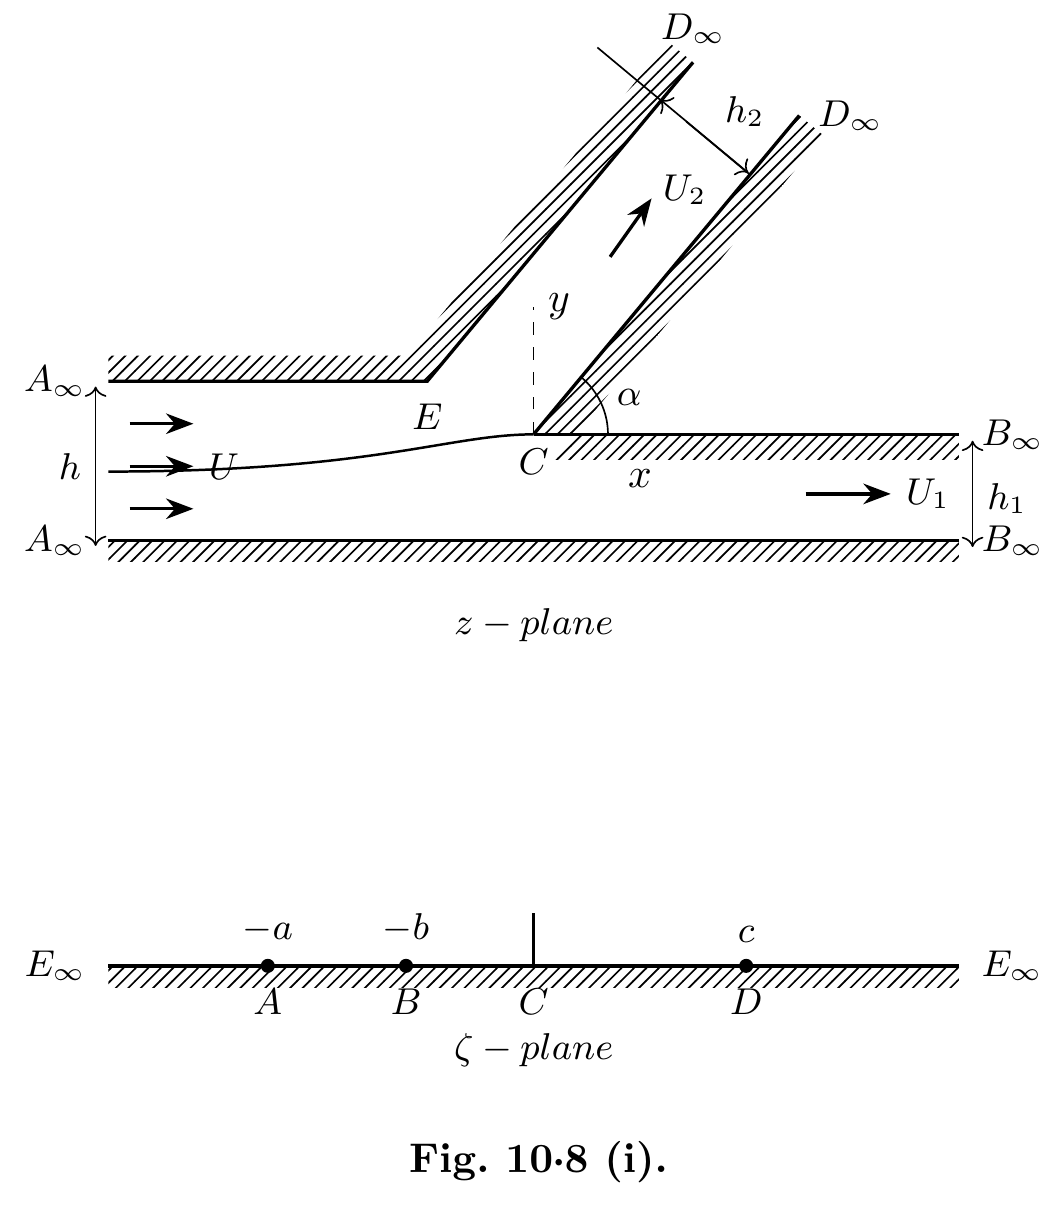
\includegraphics[width=0.62\linewidth]{1.png}
\caption{Flujo plano en una bifurcación de canal y planos $z$ y $\zeta$ del mapeo conforme.}
\label{fig:mapeo}
\Fuente{Reproducido de \citet{milnethomson1962}.}
\end{figure}

\subsection{Formulación II: energía por ramal con nivel común}\label{sec:f2}
La Formulación II sigue la ecuación de energía entre la unión y una sección terminal de cada ramal, con unión de redes tipo \citet[cap.~6]{chaudhry2008}. Para un ramal rectangular $i$ de ancho $b_i$,
\begin{equation}
G_i=H_J+(1-K_i)\frac{Q_i^2}{2gA_{J,i}^2}-(z_{d,i}+y_{d,i})-\frac{Q_i^2}{2gA_{d,i}^2}-\frac{L_i}{2}\!\left[S_{f,i}(Q_i,y_J)+S_{f,i}(Q_i,y_{d,i})\right]=0,
\label{eq:Gi}
\end{equation}
con $A_{J,i}=b_iy_J$, $A_{d,i}=b_iy_{d,i}$, $z_{d,i}=z_J-S_iL_i$, $K_i$ el coeficiente de pérdida local aplicado a la carga cinética nodal y $S_f=\left(nQ/AR^{2/3}\right)^2$ la pendiente de fricción de Manning, con $R=A/P=b_iy/(b_i+2y)$. La fricción se integra con la regla del trapecio entre los dos tirantes extremos; no se resuelve el perfil $y(x)$.

Las incógnitas son $\mathbf X=[Q_1,Q_2,H_J]^{\mathsf T}$ y el sistema normalizado es
\begin{equation}
\mathbf F(\mathbf X)=\begin{bmatrix}(Q_0-Q_1-Q_2)/Q_0\\ G_1(Q_1,H_J)/y_{\mathrm{ref}}\\ G_2(Q_2,H_J)/y_{\mathrm{ref}}\end{bmatrix}=\mathbf 0,\qquad
\mathbf J=\begin{bmatrix}-1/Q_0&-1/Q_0&0\\ G_{1,Q}/y_{\mathrm{ref}}&0&G_{1,H}/y_{\mathrm{ref}}\\ 0&G_{2,Q}/y_{\mathrm{ref}}&G_{2,H}/y_{\mathrm{ref}}\end{bmatrix},
\label{eq:sistema}
\end{equation}
con $y_{\mathrm{ref}}=1.60$ m. El ángulo $\theta$ no aparece en las ecuaciones \eqref{eq:Gi}--\eqref{eq:sistema}: con parámetros de sección, rugosidad, longitud, pendiente y calados fijos, la formulación predice el mismo reparto para todo $\theta$. Es una propiedad del modelo y no evidencia de que el ángulo carezca de efecto físico. Para dimensionar un ramal se puede añadir $b_2$ como incógnita y la restricción $Q_2=\varphi_\ast Q_0$, lo que da un sistema $4\times4$ con la misma estructura.

\subsection{Método de Newton--Raphson}
Dado $\mathbf X^{(k)}$, el paso se obtiene de $\mathbf J(\mathbf X^{(k)})\,\Delta\mathbf X=-\mathbf F(\mathbf X^{(k)})$ y la actualización $\mathbf X^{(k+1)}=\mathbf X^{(k)}+\alpha_k\Delta\mathbf X$ usa un factor de amortiguación $\alpha_k\in(0,1]$ por retroceso hasta que $\|\mathbf F\|$ decrezca \citep{chapra2015}. Con jacobiano analítico y buen punto inicial la convergencia es cuadrática cerca de la raíz. La convergencia desde un punto dado no demuestra existencia ni unicidad de la solución física.

\subsection{Sensibilidad local e incertidumbre paramétrica}
Si $\mathbf F(\mathbf X^\ast,\mathbf p)=\mathbf 0$, la diferenciación implícita da
\begin{equation}
\frac{\partial\mathbf X^\ast}{\partial p_k}=-\mathbf J^{-1}\frac{\partial\mathbf F}{\partial p_k},\qquad
E_{\varphi,p_k}=\frac{\partial\varphi}{\partial p_k}\frac{p_k}{\varphi},
\label{eq:elast}
\end{equation}
donde $E$ es la elasticidad local. Con parámetros independientes de desviación $\sigma_{p_k}$, la varianza lineal es $\sigma_\varphi^2\simeq\sum_k(\partial\varphi/\partial p_k\,\sigma_{p_k})^2$, que se contrasta con una simulación Monte Carlo \citep{saltelli2008}. Ambas son condicionales a las desviaciones postuladas y no son intervalos de confianza del desempeño real.

\subsection{Modelo 2D de HEC-RAS: ecuaciones de aguas poco profundas}\label{sec:dw}
Las ecuaciones 2D de Saint-Venant promediadas en profundidad expresan continuidad y cantidad de movimiento para el tirante $d$ y las velocidades medias $u,v$:
\begin{align}
\partial_t d+\partial_x(du)+\partial_y(dv)&=q_s,\nonumber\\
\partial_t(du)+\partial_x\!\left(du^2+\tfrac12gd^2\right)+\partial_y(duv)&=-gd\,\partial_xz_b-\tau_{b,x}/\rho,
\label{eq:swe}
\end{align}
y una ecuación análoga en $y$. HEC-RAS ofrece este sistema con dos tratamientos numéricos, SWE-ELM y SWE-EM (este último con un tratamiento más estricto de la cantidad de movimiento), además de una \emph{onda difusiva} que desprecia la aceleración local y convectiva \citep{hecmomentum,hecmanual}. En este trabajo se usa SWE-EM, elegido porque reproduce el remanso 1D en ramales angostos y diagonales (Sección~\ref{sec:verif2d}). En el formulario 2D el radio hidráulico se aproxima por el tirante local ($R\approx d$), de modo que la rugosidad efectiva de una sección angosta difiere de la que aplica un modelo 1D con perímetro mojado completo. Para medir la resistencia que el modelo produce realmente se define la rugosidad efectiva
\begin{equation}
n_\mathrm{eff}=\frac{A\,R^{2/3}\sqrt{S_f}}{Q},
\label{eq:neff}
\end{equation}
con $S_f$ la pendiente de la línea de energía simulada ($E=\zeta+V^2/2g$) entre el 15 y el 85\pc de la longitud del ramal; $n_\mathrm{eff}$ difiere del $n$ ingresado cuando la discretización añade o quita resistencia.

\subsection{Criterios de comparación}\label{sec:sesgo}
La fracción $\varphi_{2D}=Q_{2,2D}/Q_{0}$ y el error del reparto se definen por $\Delta\varphi=\varphi_{1D}-\varphi_{2D}$ y $\varepsilon(Q_2)=100\,(Q_{2,1D}-Q_{2,2D})/Q_{2,2D}$. Como referencia operativa se adoptan los umbrales de $\varepsilon(Q_2)\leq10\pc$ (aceptable) y $\leq20\pc$ (marginal), propuestos por el grupo y pendientes de confirmación por el docente; no son una norma. La verificación del modelo 2D usa una tolerancia de $\pm0.01$ m en el nivel del agua respecto del remanso 1D.

\section{Materiales y métodos}\label{sec:metodos}
\subsection{Caso sintético y datos}
El caso es sintético y no representa una obra ni un levantamiento reales. Se adopta $Q_0=12.00\,\Qs$, $g=9.81\,\mathrm{m/s^2}$ y $z_J=100.00$ m. Los anchos de fondo son $b_0=4$ m (canal principal), $b_1=3$ m y $b_2=2$ m; la Tabla~\ref{tab:datos} reúne el resto. El canal principal no interviene en las ecuaciones 1D, pero sí en la geometría 2D. Se consideran cinco ángulos entre ejes: $30^\circ$, $45^\circ$, $60^\circ$, $90^\circ$ y $120^\circ$. El esquema isométrico del canal se muestra en la Figura~\ref{fig:esquema}. Los datos están en \path{datos/datos_entrada.json}.

\begin{table}[H]
\centering\small
\caption{Datos de entrada del caso nominal.}\label{tab:datos}
\begin{tabular}{lrr}
\toprule
Parámetro & Ramal 1 & Ramal 2\\\midrule
Ancho de fondo $b$ (m) & 3.00 & 2.00\\
Longitud $L$ (m) & 200 & 150\\
Rugosidad de Manning $n$ & 0.015 & 0.018\\
Pendiente de fondo $S$ (m/m) & 0.0008 & 0.0010\\
Calado de control $y_d$ (m) & 1.60 & 1.40\\
Cota de fondo en la unión $z_J$ (m) & 100.00 & 100.00\\
Coeficiente local $K$ & 0.20 & 0.20\\\bottomrule
\end{tabular}
\Fuente{Elaboración propia (caso sintético).}
\end{table}

\begin{figure}[H]
\centering
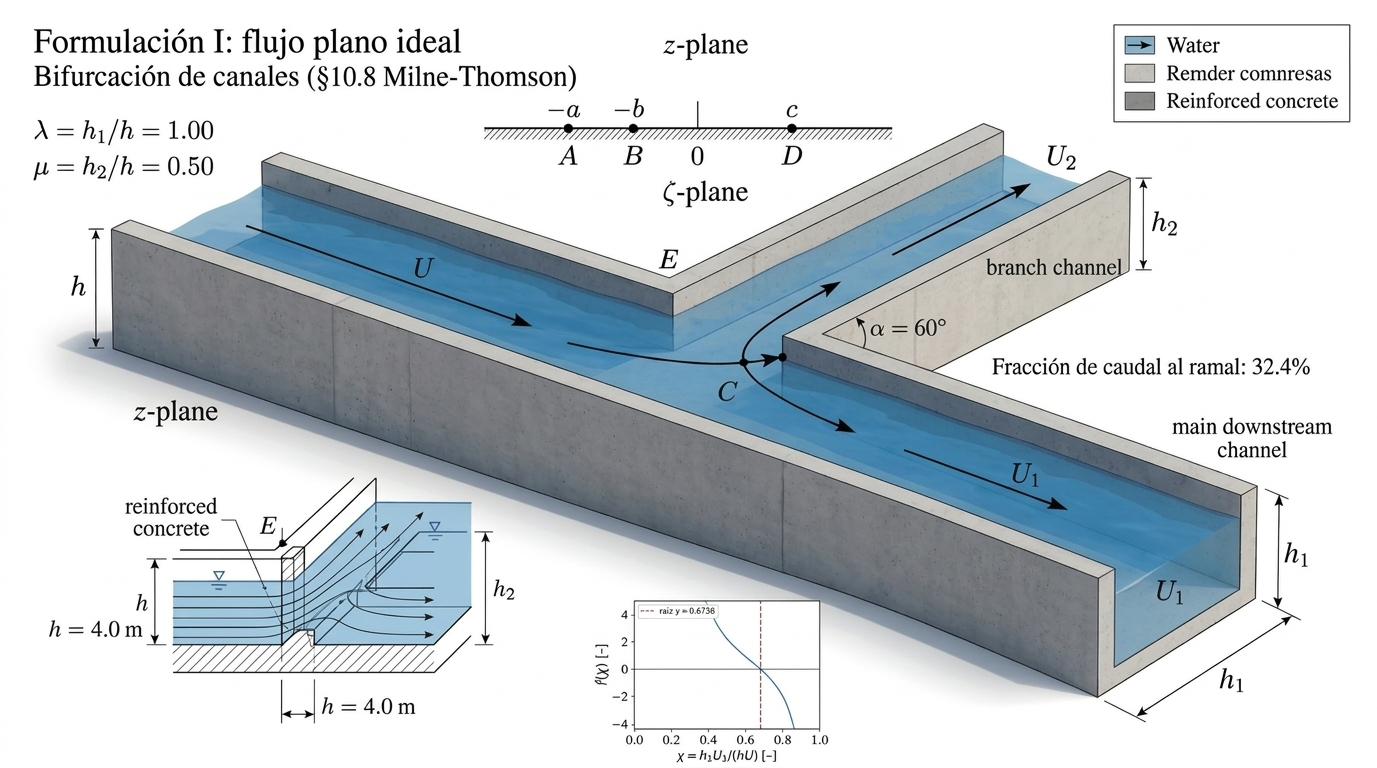
\includegraphics[width=0.82\linewidth,height=0.42\textheight,keepaspectratio]{2.png}
\caption{Esquema isométrico del canal bifurcado y nomenclatura. Ilustrativo, no a escala.}\label{fig:esquema}
\Fuente{Elaboración propia.}
\end{figure}

\subsection{Implementación numérica y reproducibilidad}
El código está en Python 3.13 con NumPy 2.5, pandas 3.0 y Matplotlib 3.11. La Formulación I se resuelve con Newton--Raphson sobre \eqref{eq:f1} para cada $\alpha$. La Formulación II usa Newton amortiguado con el jacobiano analítico \eqref{eq:sistema}, resolución del sistema lineal con \texttt{numpy.linalg.solve}, tolerancia $10^{-12}$ sobre $\|\mathbf F\|_\infty$, máximo de 50 iteraciones y retroceso hasta un factor mínimo de $10^{-4}$. El punto inicial reparte $Q_0$ según las conductancias de los ramales evaluadas con sus calados de control y coloca $H_J$ $0.05$ m sobre el mayor nivel terminal. El Monte Carlo usa 1500 realizaciones, desviaciones independientes y normales (caudal 5\pc, anchos 2\pc, Manning 10\pc, longitudes 2\pc, pendientes 5\pc, calados de control 0.04 m, $K$ 0.10 en valor absoluto) y la semilla fija \texttt{20261103}. Los resultados 1D se regeneran con \path{codigo/newton_bifurcacion.py}, que imprime las versiones de las bibliotecas y el historial de iteraciones.

\subsection{Pruebas de verificación del código}
Se aplican tres pruebas: (i) simetría analítica, con dos ramales idénticos el reparto debe ser $Q_0/2$ a cada lado; (ii) conservación de masa del caso nominal, $Q_1+Q_2-Q_0$; y (iii) contraste con una red de ocho canales publicada \citep[cap.~6]{chaudhry2008}. Además, las hojas de resultados 1D entregadas junto con el libro de HEC-RAS se contrastan con las soluciones recalculadas.

\subsection{Modelo bidimensional}\label{sec:hecras}
Las simulaciones usan los paquetes v3 del generador de geometría 2D, que reúnen los cambios derivados de las pruebas de verificación (Sección~\ref{sec:verif2d}); se ejecutaron en HEC-RAS 6.6/7.0 (unidades SI) por los tres integrantes del grupo, con la misma configuración para los cinco ángulos.
\begin{itemize}
\item \textbf{Ecuaciones:} SWE-EM (\emph{stricter momentum}), $\theta=1$, Courant adaptativo con máximo 1.0.
\item \textbf{Terreno y rugosidad:} raster de terreno y de Manning con celda de 0.05 m; $n=0.015$ en el canal principal y el ramal 1 y $n=0.018$ en el ramal 2. Canal de entrada de 50 m; las líneas de condición de borde se acortan 0.05 m por extremo y el fondo se abre 1.5 m aguas afuera de cada salida.
\item \textbf{Condiciones de borde:} hidrograma de entrada de 0.5 a $12\,\Qs$ en 600 s, mantenido hasta 7200 s; nivel fijo en las salidas (101.44 m en el ramal 1 y 101.25 m en el ramal 2), que equivale a los calados de control nominales de 1.60 y 1.40 m.
\item \textbf{Malla:} malla uniforme de 0.25 m para los cinco ángulos; en 30° y 120° se añadieron mallas de 0.50 y 0.125 m y regiones de refinamiento local en el nudo (0.125 y 0.0625 m sobre unos 90 m$^2$).
\item \textbf{Reparto:} $\varphi=Q_2/Q_0$ con los caudales de las líneas de borde de salida promediados en los últimos 600 s.
\end{itemize}
Una corrida se acepta si el error de volumen es menor que 0.5\pc, el cierre $|Q_1+Q_2-Q_0|/Q_0$ es menor que 1\pc y el caudal es estable entre los últimos 600 s y los 600 s previos (diferencia menor que 0.5\pc).

\subsection{Verificación en ramales rectos aislados}\label{sec:verif2d}
Antes de interpretar el reparto se simuló cada ramal por separado, recto, con su caudal nominal ($6.9405$ y $5.0595\,\Qs$) y su nivel de salida, y se comparó el perfil de la superficie con el remanso 1D integrado por Runge--Kutta de cuarto orden. La resistencia efectiva se calculó con \eqref{eq:neff}; el estimador devuelve $0.01500$ y $0.01795$ sobre los perfiles 1D, de modo que no tiene sesgo. Con celdas de 0.50, 0.25 y 0.125 m se obtuvo $n_\mathrm{eff}/n$ para los dos ramales. Después se probó una corrección lineal: ingresar $n/(n_\mathrm{eff}/n)$ medido a 0.25 m ($0.0174$ y $0.0212$) y comprobar que $n_\mathrm{eff}$ y el nivel recuperan los valores nominales, con tolerancia de $\pm0.01$ m.

\subsection{Conjunto exploratorio con SWE-ELM}
Un integrante ejecutó además un conjunto con SWE-ELM, celdas de 0.50, 0.25 y 0.125 m y los cinco ángulos, con un paquete anterior del generador. Los caudales se midieron en secciones transversales de los resultados. Se informa como exploratorio porque SWE-ELM no pasó la verificación en ramales diagonales estrechos y porque el paquete no incorpora las correcciones de la v3.

\subsection{Balance de masa}
El balance de volumen se tomó del resumen de cálculo de cada plan (\textit{Volume Accounting}; \citealt{hecmass}). El error relativo se define como $100\,(V_\mathrm{ent}-V_\mathrm{sal}-\Delta V_\mathrm{alm})/V_\mathrm{ent}$.

\section{Resultados}\label{sec:resultados}
\subsection{Soluciones 1D y verificación del código}
Con los datos de la Tabla~\ref{tab:datos}, la Formulación II converge a $Q_1=6.9405\,\Qs$, $Q_2=5.0595\,\Qs$ y $H_J=101.5937$ m ($y_J=1.5937$ m), es decir $\varphi=0.4216$, igual para los cinco ángulos. La Formulación I da, en cambio, un reparto que crece con el ángulo (Tabla~\ref{tab:f1}), con $\lambda=0.75$ y $\mu=0.50$. La diferencia de nivel entre ramales que exigiría el flujo ideal, $(y_1-y_2)/y$, crece de $0.45\pc$ en $30^\circ$ a $15.9\pc$ en $90^\circ$ y $32.3\pc$ en $120^\circ$.

\begin{table}[H]
\centering\small
\caption{Fracción al ramal 2 según la Formulación I.}\label{tab:f1}
\begin{tabular}{lccccc}
\toprule
$\alpha$ ($^\circ$) & 30 & 45 & 60 & 90 & 120\\\midrule
$\varphi_{\mathrm I}=Q_2/Q_0$ & 0.4063 & 0.4353 & 0.4779 & 0.6025 & 0.7845\\\bottomrule
\end{tabular}
\Fuente{Elaboración propia, Newton--Raphson sobre \eqref{eq:f1}.}
\end{table}

La convergencia de Newton--Raphson para la Formulación II se detalla en la Tabla~\ref{tab:iter}: el residuo cae de $1.2\times10^{-1}$ a $2\times10^{-15}$ en cuatro iteraciones, con el comportamiento cuadrático esperado cerca de la raíz. La Figura~\ref{fig:redes} muestra las redes de flujo de la Formulación I para $30^\circ$, $60^\circ$, $90^\circ$ y $120^\circ$ con la geometría de la Fase I del cuaderno ($\lambda=1$, $\mu=0.5$), distinta de la del caso nominal.

\begin{table}[H]
\centering\small
\caption{Historial de Newton--Raphson, Formulación II, caso nominal.}\label{tab:iter}
\begin{tabular}{rrrrr}
\toprule
Iteración & $Q_1$ ($\Qs$) & $Q_2$ ($\Qs$) & $H_J$ (m) & $\|\mathbf F\|_\infty$\\\midrule
0 & 8.823406 & 3.176594 & 101.490000 & $1.247\times10^{-1}$\\
1 & 6.717514 & 5.282486 & 101.568979 & $3.577\times10^{-2}$\\
2 & 6.936867 & 5.063133 & 101.593352 & $5.227\times10^{-4}$\\
3 & 6.940494 & 5.059506 & 101.593677 & $1.326\times10^{-7}$\\
4 & 6.940494 & 5.059506 & 101.593678 & $2.186\times10^{-15}$\\\bottomrule
\end{tabular}
\Fuente{Elaboración propia, \path{codigo/newton_bifurcacion.py}.}
\end{table}

\begin{figure}[H]
\centering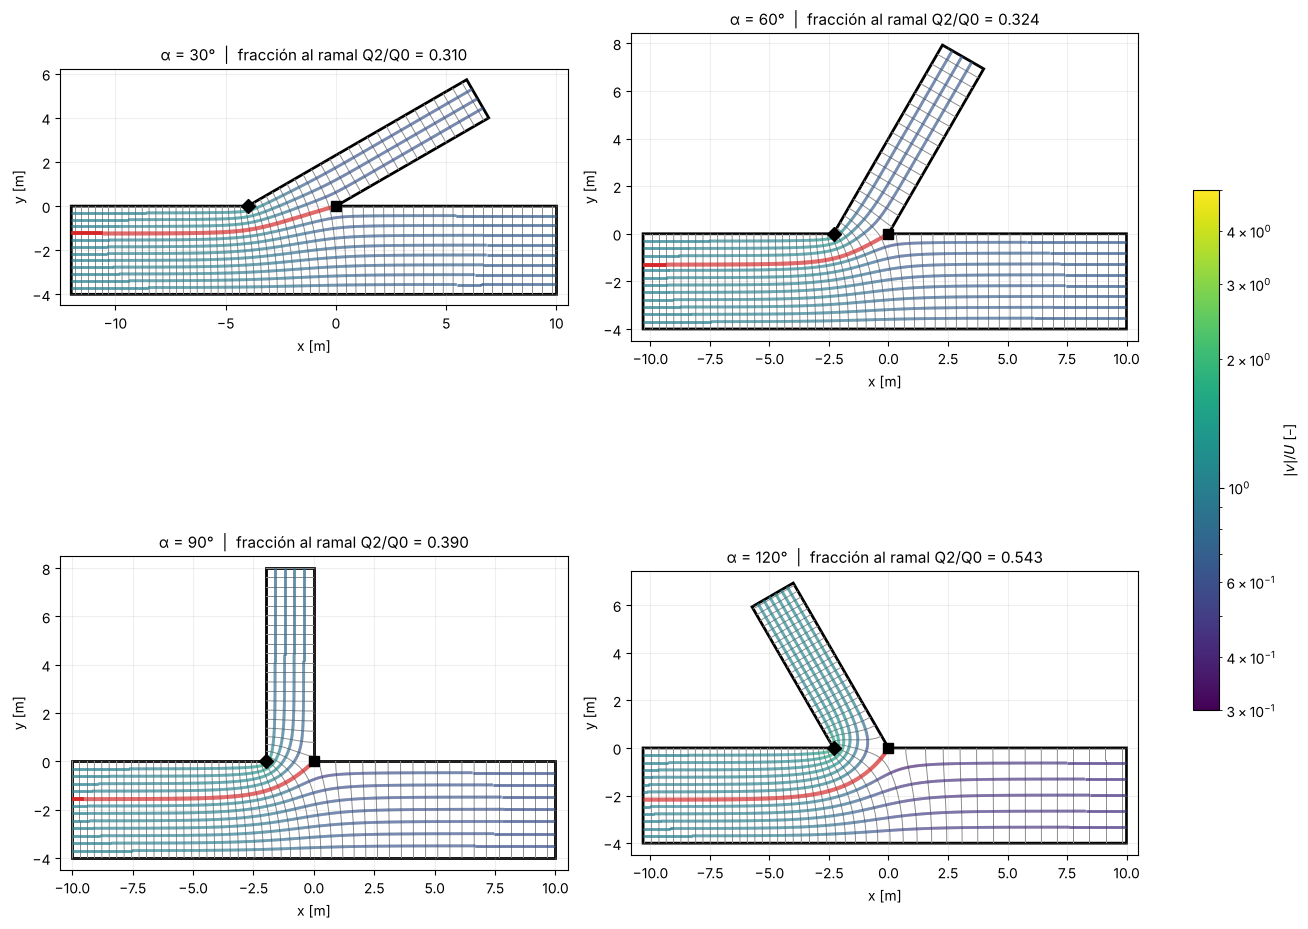
\includegraphics[width=0.92\linewidth]{3.png}
\caption{Redes de flujo de la Formulación I (potencial ideal con tapa rígida) para varios ángulos; la fracción al ramal se indica sobre cada panel.}\label{fig:redes}
\Fuente{Elaboración propia con el cuaderno de la Fase I. Los repartos indicados (0.310, 0.324, 0.390 y 0.543) corresponden a $\lambda=1$ y $\mu=0.5$ y se reprodujeron con Newton--Raphson sobre \eqref{eq:f1}; los de la Tabla~\ref{tab:f1} corresponden a $\lambda=0.75$ y $\mu=0.50$.}
\end{figure}

La Tabla~\ref{tab:verif} resume las pruebas. El benchmark de la red de ocho canales \emph{no se reproduce}: la reconstrucción difiere hasta 33.3\pc (10.5 $\Qs$) de los valores tabulados, y varios calados de esa red se excluyeron por inconsistencias internas. Se reporta como prueba no superada; no se afirma que el código de la red esté validado.

\begin{table}[H]
\centering\small
\caption{Pruebas de verificación.}\label{tab:verif}
\begin{tabular}{>{\raggedright\arraybackslash}p{0.34\linewidth}>{\raggedright\arraybackslash}p{0.34\linewidth}>{\raggedright\arraybackslash}p{0.14\linewidth}}
\toprule
Prueba & Resultado & Estado\\\midrule
Simetría, ramales idénticos & $Q_1=Q_2=2.0000\,\Qs$; error 0 (tolerancia $10^{-10}$) & Cumple\\
Conservación de masa, caso nominal & $Q_1+Q_2-Q_0=0.0000$ & Cumple\\
Hoja 1D del 90° vs. Formulación II & Coincide ($Q_1=6.9405$, $Q_2=5.0595$) & Cumple\\
Hoja de Milne-Thomson vs. Formulación I & Diferencia máx. $|\Delta\varphi|=4.5\times10^{-7}$ & Cumple\\
Red de ocho canales (Chaudhry) & Diferencia relativa máx. 33.3\pc & No cumple\\\bottomrule
\end{tabular}
\end{table}

\subsection{Sensibilidad del reparto}
La Figura~\ref{fig:elast} muestra las elasticidades de $\varphi$ para los 13 parámetros, evaluadas en las configuraciones del conjunto exploratorio inicial (calados de salida del 2D de entonces). Dominan los calados de control ($|E|\approx0.8$ a $1.3$, con signo opuesto entre ramales), los anchos de fondo ($|E|\approx0.75$ a $0.96$) y la rugosidad ($|E|\approx0.5$). El caudal total, las longitudes y el coeficiente local tienen efecto pequeño ($|E|\leq0.26$; $|E(K)|\approx0.03$). La incertidumbre postulada produce $\sigma_\varphi=0.031$ a $0.036$ en la aproximación lineal y $0.033$ a $0.037$ en Monte Carlo, con diferencias de $-0.4$ a $+7.6\pc$ entre ambos métodos, de modo que la linealización es adecuada.

\begin{figure}[H]
\centering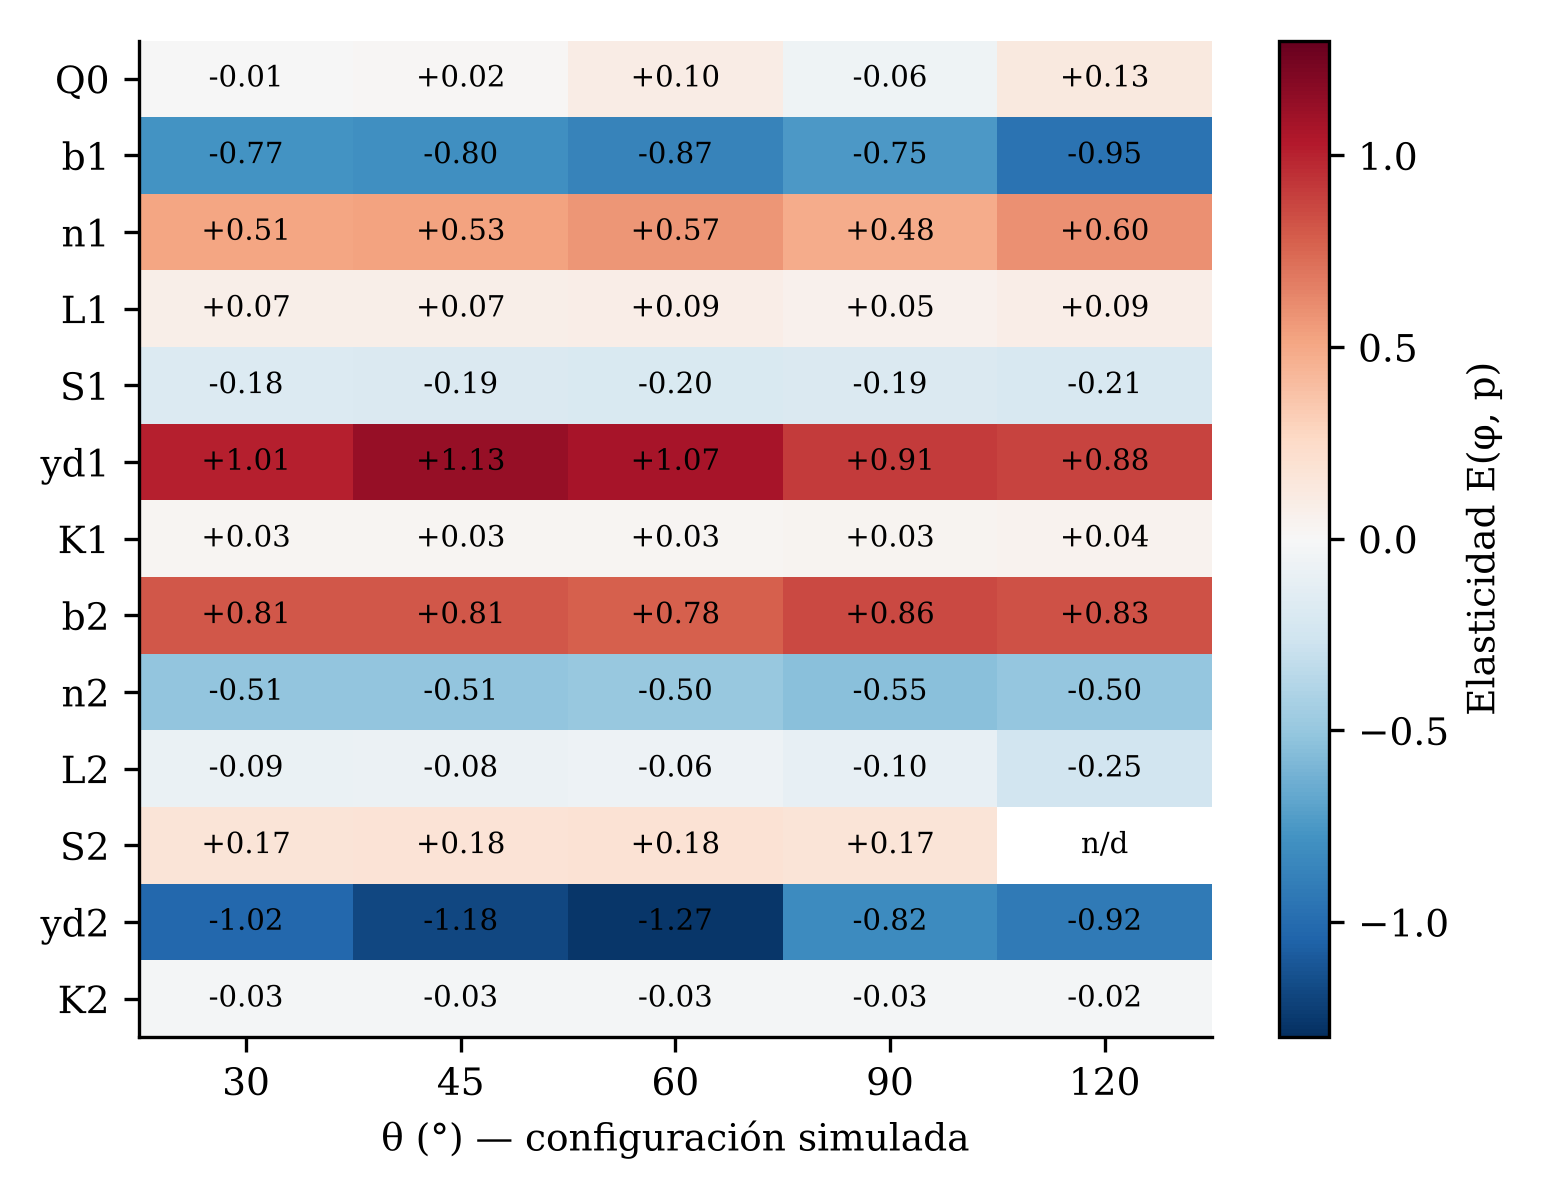
\includegraphics[width=0.62\linewidth]{fig_elasticidad.png}
\caption{Elasticidades de $\varphi$ por ángulo (configuraciones del conjunto exploratorio inicial). Para $120^\circ$, $S_2=0$ y la elasticidad de $S_2$ no está definida.}\label{fig:elast}
\Fuente{Elaboración propia, cuaderno de la Fase IV.}
\end{figure}

\subsection{Sensibilidad de la Formulación II a $K$ y a $n$}
Dos parámetros se barren aparte porque son los que se discuten al comparar con el 2D (Tabla~\ref{tab:barrido}). La pérdida local $K$ casi no mueve el reparto: de $K=0$ a $2.4$, $\varphi$ pasa de $0.4232$ a $0.4142$ (diferencia $0.009$). En cambio, \emph{reducir} la rugosidad en ambos ramales \emph{aumenta} $\varphi$ ($0.4741$ con $n$ al 72\pc del nominal), de modo que una resistencia efectiva menor en el 2D no puede explicar un reparto menor.

\begin{table}[H]
\centering\small
\caption{Reparto de la Formulación II al variar $K$ (con $n$ nominal) y al escalar $n$ en ambos ramales (con $K=0.2$).}\label{tab:barrido}
\begin{tabular}{lccccc}
\toprule
$K$ & 0 & 0.2 & 0.5 & 1 & 2.4\\
$\varphi_\mathrm{II}$ & 0.4232 & 0.4216 & 0.4198 & 0.4176 & 0.4142\\\midrule
$n/n_\mathrm{nom}$ & 1.00 & 0.93 & 0.86 & 0.72 & \\
$\varphi_\mathrm{II}$ & 0.4216 & 0.4314 & 0.4430 & 0.4741 & \\\bottomrule
\end{tabular}
\Fuente{Elaboración propia, \path{codigo/newton_bifurcacion.py} con los datos de la Tabla~\ref{tab:datos}.}
\end{table}

\subsection{Verificación del 2D en ramales rectos aislados}\label{sec:resverif}
Con SWE-EM y celda de 0.25 m el nivel simulado sigue el remanso 1D con diferencias de pocos centímetros, pero la resistencia efectiva depende de la malla: $n_\mathrm{eff}/n=0.93$, $0.86$ y $0.72$ para celdas de 0.50, 0.25 y 0.125 m, con el mismo valor en los dos ramales (Tabla~\ref{tab:neff}); aproximadamente $n_\mathrm{eff}/n\approx1-0.035/\Delta x$. En el ramal 2 del nudo a $30^\circ$ la tendencia con la malla es la contraria ($n_\mathrm{eff}$ de $0.0183$ a $0.0233$ al refinar), de modo que la geometría diagonal añade una resistencia propia del modelo.

\begin{table}[H]
\centering\small
\caption{Resistencia efectiva en ramales rectos aislados (SWE-EM).}\label{tab:neff}
\begin{tabular}{cc}
\toprule
Celda (m) & $n_\mathrm{eff}/n$\\\midrule
0.50 & 0.93\\
0.25 & 0.86\\
0.125 & 0.72\\\bottomrule
\end{tabular}
\Fuente{Elaboración propia con los resultados HDF de los ramales aislados.}
\end{table}

La corrección lineal \emph{no cumple} la comprobación (Tabla~\ref{tab:correccion}). Con $n$ de entrada $0.0174$ en el ramal 1 se obtiene $n_\mathrm{eff}=0.0143$ (objetivo $0.0150$) y un error máximo de nivel de $0.018$ m; con $0.0212$ en el ramal 2 se obtiene $0.0170$ (objetivo $0.0180$) y $0.041$ m. Los niveles siguen por debajo del 1D, es decir, aún falta resistencia: la respuesta del modelo a $n$ no es lineal ($n_\mathrm{eff}/n_\mathrm{entrada}$ baja de $0.86$ a $0.82$). Por eso la corrección se reporta solo como diagnóstico y no se aplicó a las corridas del nudo.

\begin{table}[H]
\centering\small
\caption{Prueba de corrección de $n$ (celda 0.25 m).}\label{tab:correccion}
\begin{tabular}{lccccc}
\toprule
Ramal & $n$ entrada & $n_\mathrm{eff}$ objetivo & $n_\mathrm{eff}$ obtenido & Error máx. de nivel (m) & Criterio ($\pm0.01$ m)\\\midrule
1 & 0.0174 & 0.0150 & 0.0143 & 0.018 & No cumple\\
2 & 0.0212 & 0.0180 & 0.0170 & 0.041 & No cumple\\\bottomrule
\end{tabular}
\Fuente{Elaboración propia con los resultados HDF de los ramales aislados (planes con $n$ corregido).}
\end{table}

\subsection{Control de calidad de las corridas del nudo}
Las cinco corridas con celda de 0.25 m cumplen los criterios de aceptación (Tabla~\ref{tab:cc}): error de volumen entre $2.7\times10^{-6}$ y $8.9\times10^{-3}\pc$, cierre de caudal $\leq0.009\pc$ y reparto idéntico entre los últimos 600 s y los 600 s previos. En $90^\circ$ el cálculo informa un error máximo de nivel de celda de 0.62 m en una celda aislada junto a la punta de la divisoria (a $x\approx-0.1$ m, $y\approx2.1$ m del nudo), sin efecto sobre el volumen ni sobre los caudales.

\begin{table}[H]
\centering\small
\caption{Control de calidad de las corridas SWE-EM con celda de 0.25 m.}\label{tab:cc}
\begin{tabular}{rcccc}
\toprule
$\theta$ ($^\circ$) & Celdas & Error de volumen (\%) & Cierre de caudal (\%) & $\varphi$ última 600 s / previa\\\midrule
30 & 20174 & $3.1\times10^{-6}$ & 0.000 & 0.3739 / 0.3739\\
45 & 23092 & $8.9\times10^{-3}$ & 0.009 & 0.3581 / 0.3581\\
60 & 20207 & $3.1\times10^{-6}$ & 0.000 & 0.3503 / 0.3503\\
90 & 24108 & $7.1\times10^{-4}$ & 0.001 & 0.3402 / 0.3402\\
120 & 20248 & $2.7\times10^{-6}$ & 0.000 & 0.3132 / 0.3132\\\bottomrule
\end{tabular}
\Fuente{Elaboración propia, resúmenes de cálculo y series de caudal de los planes HDF.}
\end{table}

\subsection{Reparto: contraste 1D--2D}
La Tabla~\ref{tab:reparto} y la Figura~\ref{fig:phitheta} contrastan las formulaciones con el 2D. El 2D da un reparto que \emph{decrece} con el ángulo, de $0.374$ a $0.313$. La Formulación I crece de $0.406$ a $0.785$: acierta en magnitud a $30^\circ$ ($+8.7\pc$) pero se aleja con el ángulo hasta $+150\pc$ a $120^\circ$, con tendencia opuesta. La Formulación II es constante en $0.4216$ y sobrestima $Q_2$ entre $+12.8$ y $+34.6\pc$, con un error que crece con $\theta$. Con el conjunto exploratorio SWE-ELM de 0.125 m, el reparto es $\approx0.41$ entre $30^\circ$ y $60^\circ$ y la II queda a $+2.2$ a $+2.9\pc$, pero a $90^\circ$ y $120^\circ$ la brecha sube a $+11.2$ y $+28.7\pc$.

\begin{table}[H]
\centering\small
\caption{Reparto $\varphi=Q_2/Q_0$ del 2D y de las formulaciones; $\varepsilon(Q_2)$ (\%) entre paréntesis.}\label{tab:reparto}
\begin{tabular}{rccccc}
\toprule
$\theta$ ($^\circ$) & 2D SWE-EM 0.25 m & Form. I & Form. II & 2D SWE-ELM 0.125 m & II vs. ELM\\\midrule
30 & 0.3739 & 0.4063 (+8.7) & 0.4216 (+12.8) & 0.4107 & (+2.7)\\
45 & 0.3581 & 0.4353 (+21.6) & 0.4216 (+17.7) & 0.4124 & (+2.2)\\
60 & 0.3503 & 0.4779 (+36.4) & 0.4216 (+20.4) & 0.4096 & (+2.9)\\
90 & 0.3402 & 0.6025 (+77.1) & 0.4216 (+23.9) & 0.3790 & (+11.2)\\
120 & 0.3132 & 0.7845 (+150.5) & 0.4216 (+34.6) & 0.3275 & (+28.7)\\\bottomrule
\end{tabular}
\Nota{En las columnas de las formulaciones, $\varepsilon(Q_2)$ se calcula respecto del 2D SWE-EM; la última columna, respecto del 2D SWE-ELM. SWE-ELM es exploratorio (Sección~\ref{sec:hecras}). Fuente: elaboración propia.}
\end{table}

\begin{figure}[H]
\centering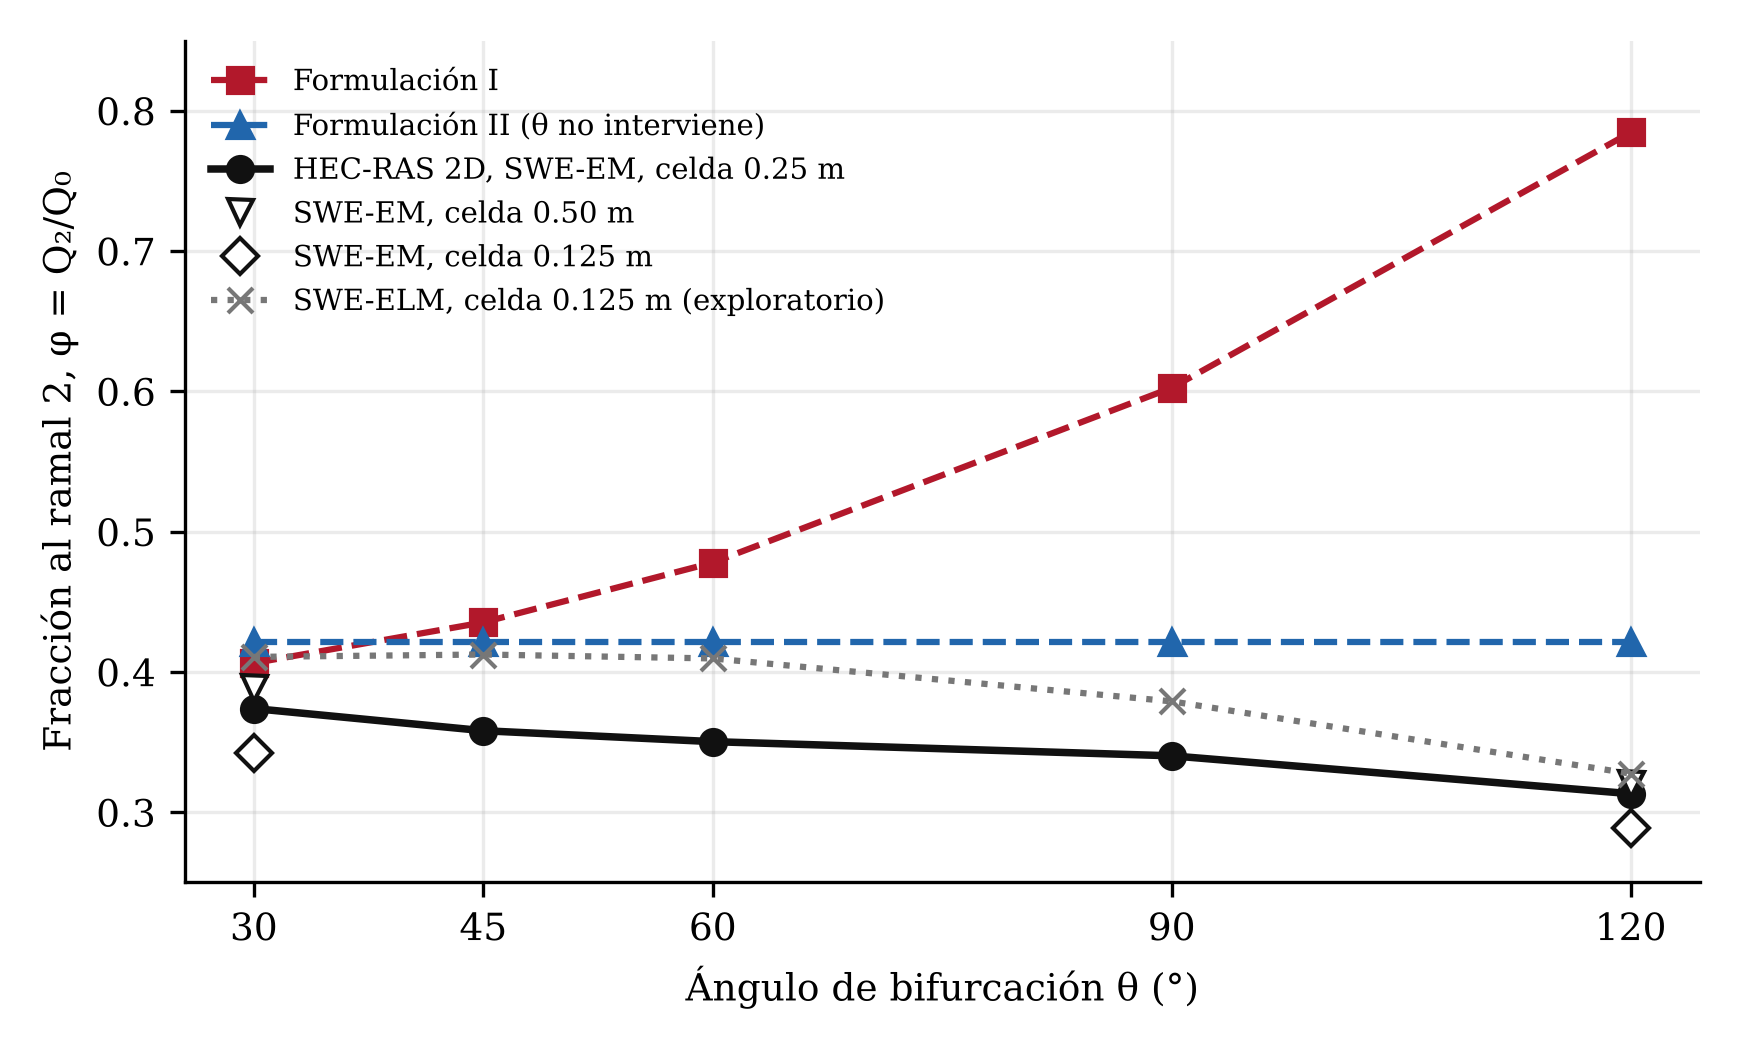
\includegraphics[width=0.78\linewidth]{fig_phi_theta.png}
\caption{Fracción al ramal 2 en función del ángulo. Los marcadores vacíos muestran la dispersión por malla del SWE-EM en 30° y 120°.}\label{fig:phitheta}
\Fuente{Elaboración propia (\path{datos/resultados_2d_v3.csv}, \path{datos/mallas_EM.csv}, \path{datos/mallas_ELM.csv}).}
\end{figure}

\subsection{Dependencia de la malla y de las ecuaciones}
En SWE-EM, $\varphi$ \emph{no converge} al refinar (Tabla~\ref{tab:mallas}, Figura~\ref{fig:malla}a): a $30^\circ$ baja de $0.389$ a $0.374$ y a $0.343$ para celdas de 0.50, 0.25 y 0.125 m, con diferencias crecientes ($0.015$ y $0.031$); a $120^\circ$ baja de $0.320$ a $0.313$ y a $0.289$. Como las diferencias crecen, no corresponde aplicar el GCI ni la extrapolación de Richardson. En cambio, refinar solo el nudo sobre la malla de 0.25 m cambia poco el resultado ($0.378$ y $0.379$ a $30^\circ$; $0.317$ y $0.316$ a $120^\circ$): la resolución local del nudo está convergida y la dependencia viene de la malla de los ramales y del canal, coherente con la pérdida de resistencia efectiva de la Sección~\ref{sec:resverif}. La corrida uniforme de 0.125 m en $120^\circ$ presenta un error de volumen mayor ($4.8\times10^{-3}\pc$) y un cierre de $0.09\pc$, todavía aceptables.

Con SWE-ELM (Figura~\ref{fig:malla}b) el reparto cambia menos con la malla entre 0.25 y 0.125 m ($\leq0.007$ en 30°, 45° y 60°), pero difiere del de SWE-EM en $0.04$ a $0.07$ a igual malla de 0.125 m.

\begin{table}[H]
\centering\small
\caption{Reparto $\varphi$ del 2D SWE-EM según la malla (30° y 120°).}\label{tab:mallas}
\begin{tabular}{llccc}
\toprule
$\theta$ ($^\circ$) & Malla & Celdas & $\varphi$ & Error de volumen (\%)\\\midrule
30 & uniforme 0.50 m & 5372 & 0.3888 & $1.7\times10^{-8}$\\
30 & uniforme 0.25 m & 20174 & 0.3739 & $3.1\times10^{-6}$\\
30 & uniforme 0.125 m & 88440 & 0.3425 & $3.0\times10^{-6}$\\
30 & 0.25 m + nudo 0.125 m & 23198 & 0.3778 & $3.1\times10^{-6}$\\
30 & 0.25 m + nudo 0.0625 m & 35239 & 0.3789 & $3.1\times10^{-6}$\\
120 & uniforme 0.50 m & 5884 & 0.3204 & $1.8\times10^{-6}$\\
120 & uniforme 0.25 m & 20248 & 0.3132 & $2.7\times10^{-6}$\\
120 & uniforme 0.125 m & 88770 & 0.2886 & $4.8\times10^{-3}$\\
120 & 0.25 m + nudo 0.125 m & 23459 & 0.3174 & $2.7\times10^{-6}$\\
120 & 0.25 m + nudo 0.0625 m & 36044 & 0.3159 & $2.7\times10^{-6}$\\\bottomrule
\end{tabular}
\Fuente{Elaboración propia, planes HDF.}
\end{table}

\begin{figure}[H]
\centering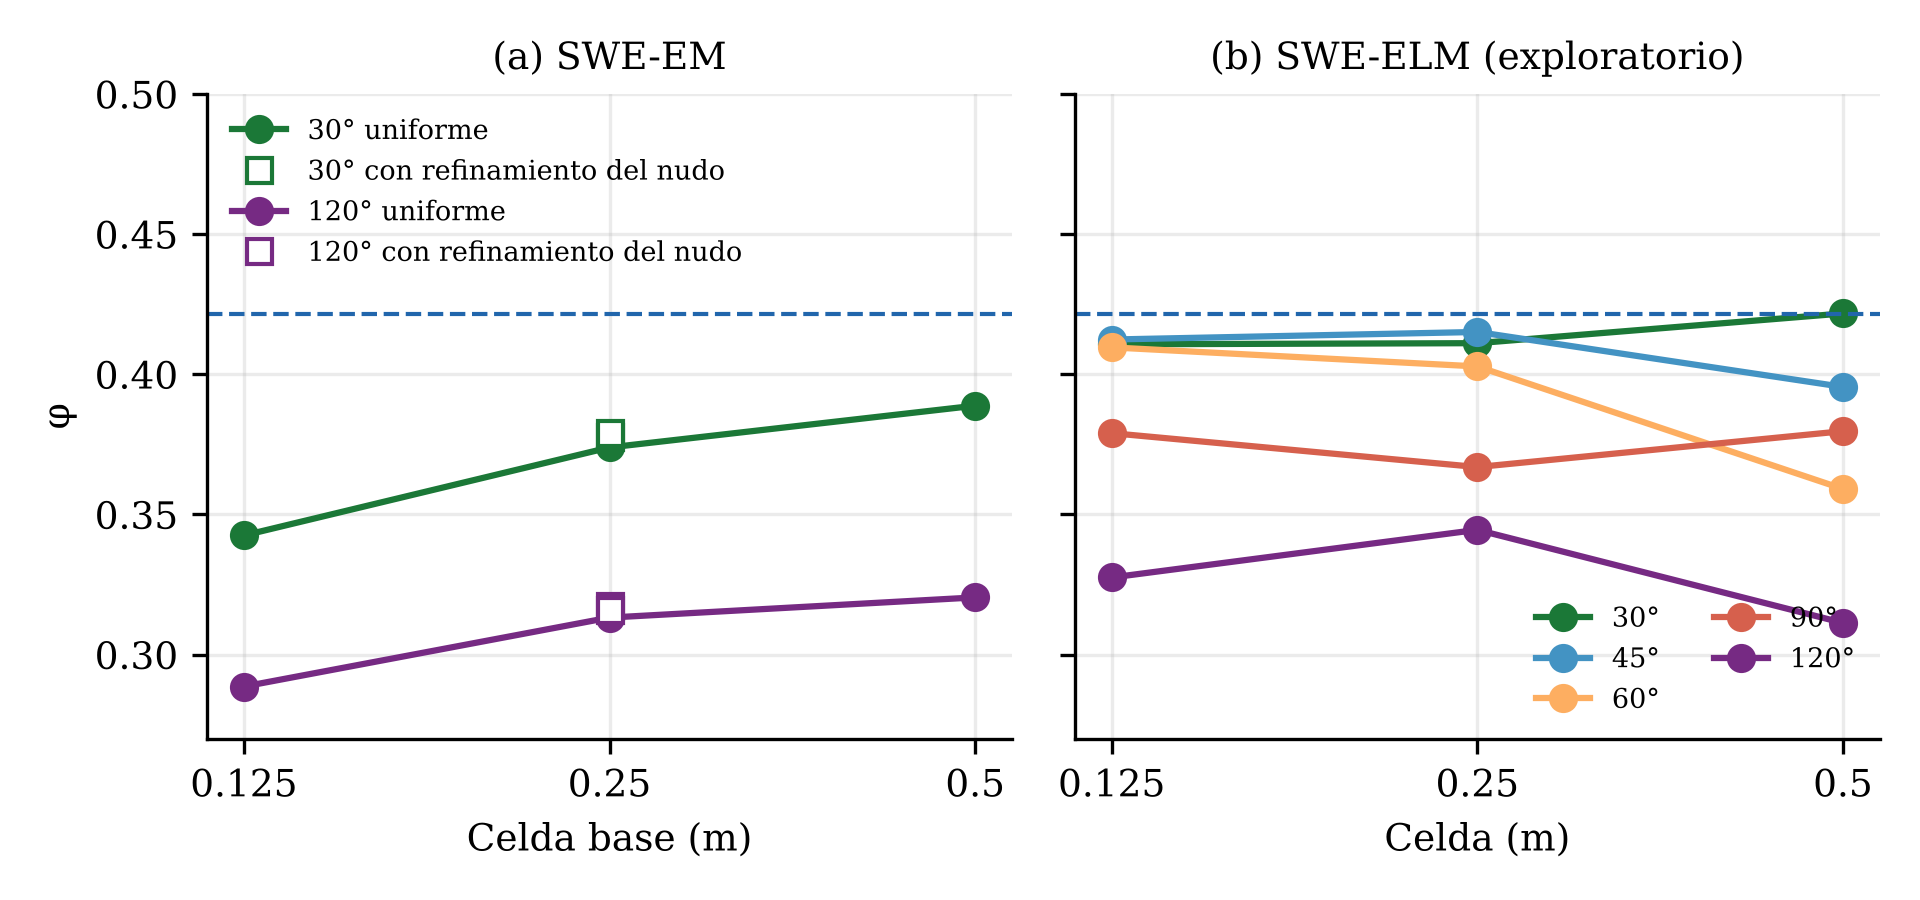
\includegraphics[width=0.92\linewidth]{fig_malla.png}
\caption{Reparto frente al tamaño de celda. (a) SWE-EM, 30° y 120°, con refinamiento local del nudo; (b) SWE-ELM, cinco ángulos. La línea discontinua es $\varphi_\mathrm{II}=0.4216$.}\label{fig:malla}
\Fuente{Elaboración propia.}
\end{figure}

\subsection{Energía en el nudo}
El balance de energía entre el canal principal y el inicio del ramal 2 en el 2D muestra una pérdida de carga que crece con el ángulo: unos $0.04$ m a $30^\circ$ y unos $0.22$ m a $120^\circ$, lo que corresponde a un coeficiente local efectivo $K_\mathrm{ef}\approx0.4$ a $0.5$ y $\approx2.4$ frente al $K=0.2$ fijo de la Formulación II (valores aproximados, malla de 0.25 m). Sin embargo, la Tabla~\ref{tab:barrido} indica que $\varphi_\mathrm{II}$ casi no responde a $K$ (de $0.4232$ a $0.4142$ para $K$ entre 0 y 2.4), de modo que un $K$ dependiente del ángulo no basta, por sí solo, para reproducir el descenso del reparto.

\section{Discusión}\label{sec:discusion}
\subsection{Por qué la Formulación I no sirve como predictor aquí}
La Formulación I no tiene condición aguas abajo ni fricción, así que su reparto es función exclusiva del ángulo y de los anchos. En el 2D el reparto decrece con el ángulo en todos los conjuntos corridos (SWE-EM entre $0.374$ y $0.313$; SWE-ELM entre $0.411$ y $0.328$), mientras que la Formulación I crece hasta $0.785$. La contradicción no depende de la malla ni de las ecuaciones del 2D, porque la brecha a $120^\circ$ (más de $0.45$) supera con holgura la dispersión entre mallas ($\leq0.03$ en SWE-EM). Es coherente con la teoría: el modelo de tapa rígida es una referencia analítica de $Fr\to0$, no un predictor para un canal con fricción y condiciones aguas abajo \citep{batchelor1967,milnethomson1962}.

\subsection{Qué reproduce y qué no reproduce la Formulación II}
La Formulación II predice $\varphi=0.4216$ para cualquier ángulo. El 2D, en cambio, muestra un descenso monótono con $\theta$ (de $0.374$ a $0.313$ con SWE-EM), de modo que la formulación no captura la tendencia por construcción. Su nivel absoluto depende de qué 2D se tome como referencia: queda a $+13\pc$ (30°) hasta $+35\pc$ (120°) del SWE-EM de 0.25 m, y a $+2$ a $+3\pc$ del SWE-ELM de 0.125 m entre 30° y 60°. Esa diferencia entre referencias es del mismo orden que la brecha que se quiere explicar, por lo que no se puede afirmar con estos datos que la Formulación II acierte el nivel del reparto en ángulos pequeños.

Los barridos de la Formulación II indican además que ni la pérdida local ni la resistencia efectiva cierran la brecha con el SWE-EM: $K$ de 0 a 2.4 mueve $\varphi$ solo $0.009$, y reducir $n$ (lo que hace el 2D al refinar) \emph{eleva} $\varphi$ en lugar de bajarlo. Lo que el 2D muestra en el nudo es una pérdida de carga hacia el ramal 2 que crece con el ángulo (unos $0.04$ m a $30^\circ$ y $0.22$ m a $120^\circ$), asociada a la separación del flujo en la esquina, y que un coeficiente $K$ aplicado a la altura de velocidad no representa. Se interpreta como una hipótesis: faltan simulaciones que aíslen el mecanismo.

\subsection{Dependencia de malla y de ecuaciones del 2D}
El SWE-EM reproduce el remanso 1D en ramales rectos y diagonales, pero su resistencia efectiva decae al refinar ($n_\mathrm{eff}/n$ de $0.93$ a $0.72$) y el reparto no converge. La corrección lineal de $n$ no cumple la tolerancia ($0.018$ y $0.041$ m de error de nivel), de modo que la dependencia de malla no se resolvió. Refinar solo el nudo no cambia el reparto, lo que ubica la sensibilidad en la fricción de los ramales y no en la resolución de la esquina. Con SWE-ELM el reparto varía menos con la malla, pero ese conjunto no pasó la verificación en ramales diagonales; que ambos conjuntos difieran en $0.04$ a $0.07$ a igual celda impide tomar cualquiera de ellos como verdad de referencia.

\subsection{Limitaciones}
\begin{enumerate}[label=\arabic*)]
\item \textbf{Malla.} Con SWE-EM, $\varphi$ no converge al refinar; las corridas de los cinco ángulos se hicieron solo con celda de 0.25 m. Las mallas de 0.50 y 0.125 m existen en 30° y 120°.
\item \textbf{Ecuaciones.} El conjunto SWE-ELM, con tres mallas y cinco ángulos, usa un paquete anterior, midió caudales en secciones transversales y no pasó la verificación en ramales diagonales; se presenta como exploratorio.
\item \textbf{Resistencia.} La resistencia efectiva del 2D difiere de la nominal y depende de la malla; la corrección lineal de $n$ no cumple $\pm0.01$ m. Las estimaciones del balance de energía son aproximadas.
\item \textbf{Sensibilidad.} Las elasticidades y la incertidumbre paramétrica ($\sigma_\varphi\approx0.035$) provienen de configuraciones del conjunto exploratorio inicial y de desviaciones postuladas por el grupo, sin datos observados.
\item \textbf{Sin validación física.} No hay datos de laboratorio ni de campo. El benchmark de la red de ocho canales no se reproduce.
\item \textbf{Alcance geométrico.} Un solo caso sintético; $K$ fijo y resultados válidos para $b_0=4$ m, $b_1=3$ m y $b_2=2$ m.
\item \textbf{Criterios.} Los umbrales de $10\pc$ y $20\pc$ son propuestos por el grupo y no una norma.
\end{enumerate}

\section{Conclusiones}\label{sec:conclusiones}
\begin{enumerate}[label=\arabic*)]
\item La Formulación II (energía por ramal con nivel común) se resuelve de forma estable por Newton--Raphson con jacobiano analítico y da $Q_2/Q_0=0.4216$ con los datos nominales, independiente del ángulo por construcción y casi insensible a la pérdida local $K$.
\item En el HEC-RAS 2D con SWE-EM y celda de 0.25 m, las cinco corridas cumplen el control de calidad (error de volumen $\leq0.009\pc$) y dan $\varphi=0.374$, $0.358$, $0.350$, $0.340$ y $0.313$ entre $30^\circ$ y $120^\circ$: el reparto decrece con el ángulo.
\item La Formulación I queda contradicha a ángulos grandes: crece de $0.406$ a $0.785$ mientras el 2D decrece, en todos los conjuntos y mallas probados.
\item La Formulación II no reproduce la tendencia con el ángulo y sobrestima $Q_2$ entre $+13$ y $+35\pc$ respecto del SWE-EM de 0.25 m; frente al conjunto exploratorio SWE-ELM de 0.125 m queda a $+2$ a $+3\pc$ entre $30^\circ$ y $60^\circ$ y a $+11$ y $+29\pc$ en $90^\circ$ y $120^\circ$.
\item El 2D no es una referencia convergida: la resistencia efectiva cae al refinar ($n_\mathrm{eff}/n=0.93$, $0.86$, $0.72$), $\varphi$ a 30° pasa de $0.389$ a $0.343$ y la corrección lineal de $n$ no cumple $\pm0.01$ m. El refinamiento local del nudo sí está convergido.
\item Lo que queda por hacer: repetir 45°, 60° y 90° con otras mallas, resolver la dependencia de la resistencia efectiva con la malla, y contrastar con datos físicos antes de recomendar una formulación 1D para el diseño.
\end{enumerate}

\vspace{8pt}
\noindent\textbf{Contribución de los autores:} \textit{[completar con los roles de cada integrante (conceptualización, software, validación, redacción, etc.)]}.

\noindent\textbf{Financiamiento:} esta investigación no recibió financiamiento externo \textit{[confirmar]}.

\noindent\textbf{Disponibilidad de datos:} los datos de entrada, los resultados tabulados, las figuras y el código para regenerarlas están en el repositorio público \repo{}, junto con los proyectos y salidas de HEC-RAS y el cuaderno de procesamiento (carpetas \path{datos/}, \path{codigo/} y de anexos). La semilla del Monte Carlo es 20261103.

\noindent\textbf{Uso de inteligencia artificial:} se utilizó una herramienta de inteligencia artificial como apoyo para organizar la redacción, desarrollar el código de cálculo y generar los cuadernos y figuras. Las ecuaciones, las hipótesis, los resultados y las referencias deben ser verificados y comprendidos por el grupo antes de la entrega (Anexo~\ref{anx:ia}). La herramienta no sustituye la responsabilidad académica de los autores.

\noindent\textbf{Conflictos de interés:} los autores declaran no tener conflictos de interés \textit{[confirmar]}.

\begin{thebibliography}{99}

\bibitem[Batchelor(1967)]{batchelor1967}
Batchelor, G. K. (1967). \emph{An introduction to fluid dynamics}. Cambridge University Press.

\bibitem[Chaudhry(2008)]{chaudhry2008}
Chaudhry, M. H. (2008). \emph{Open-channel flow} (2nd ed.). Springer. \url{https://doi.org/10.1007/978-0-387-68648-6}

\bibitem[Ghostine et al.(2012)]{ghostine2012}
Ghostine, R., Vazquez, J., Terfous, A., Mosé, R., \& Ghenaim, A. (2012). Comparative study of 1D and 2D flow simulations at open-channel junctions. \emph{Journal of Hydraulic Research, 50}(2), 164--170. \url{https://doi.org/10.1080/00221686.2012.661563}

\bibitem[Gumgum(2025)]{gumgum2025}
Gumgum, F. (2025). Division of flow at open channel bifurcations. \emph{Physics of Fluids, 37}(2), 021301. \url{https://doi.org/10.1063/5.0246741}

\bibitem[Gumgum(2026)]{gumgum2026}
Gumgum, F. (2026). Numerical Investigation of Flow Division at Lateral Diversions. \emph{Applied Sciences, 16}(7), 3239. \url{https://doi.org/10.3390/app16073239}

\bibitem[Gurevich(1965)]{gurevich1965}
Gurevich, M. I. (1965). \emph{The theory of jets in an ideal fluid}. Academic Press.

\bibitem[Hsu et al.(2002)]{hsu2002}
Hsu, C. C., Tang, C. J., Lee, W. J., \& Shieh, M. Y. (2002). Subcritical 90° equal-width open-channel dividing flow. \emph{Journal of Hydraulic Engineering, 128}(7), 716--720. \url{https://doi.org/10.1061/(ASCE)0733-9429(2002)128:7(716)}

\bibitem[Ibrahim et al.(2022)]{ibrahim2022}
Ibrahim, I., Rivière, N., Lebouteiller, I., \& Mignot, E. (2022). Discharge distribution in open-channel T-shape bifurcations: Effect of a reduced side branch width. \emph{Journal of Hydraulic Engineering, 148}(9), 04022015. \url{https://doi.org/10.1061/(ASCE)HY.1943-7900.0002002}

\bibitem[Milne-Thomson(1962)]{milnethomson1962}
Milne-Thomson, L. M. (1962). \emph{Theoretical hydrodynamics} (4th ed., reprint). Macmillan.

\bibitem[Momplot et al.(2017)]{momplot2017}
Momplot, A., Lipeme Kouyi, G., Mignot, E., Rivière, N., \& Bertrand-Krajewski, J.-L. (2017). Typology of the flow structures in dividing open channel flows. \emph{Journal of Hydraulic Research, 55}(1), 63--71. \url{https://doi.org/10.1080/00221686.2016.1212409}

\bibitem[Ramamurthy and Satish(1988)]{ramamurthy1988}
Ramamurthy, A. S., \& Satish, M. G. (1988). Division of flow in short open channel branches. \emph{Journal of Hydraulic Engineering, 114}(4), 428--438. \url{https://doi.org/10.1061/(ASCE)0733-9429(1988)114:4(428)}

\bibitem[Ramamurthy et al.(1990)]{ramamurthy1990}
Ramamurthy, A. S., Tran, D. M., \& Carballada, B. L. (1990). Dividing flow in open channels. \emph{Journal of Hydraulic Engineering, 116}(3), 449--455. \url{https://doi.org/10.1061/(ASCE)0733-9429(1990)116:3(449)}

\bibitem[Ramamurthy et al.(2007)]{ramamurthy2007}
Ramamurthy, A. S., Qu, J., \& Vo, D. (2007). Numerical and experimental study of dividing open-channel flows. \emph{Journal of Hydraulic Engineering, 133}(10), 1135--1144. \url{https://doi.org/10.1061/(ASCE)0733-9429(2007)133:10(1135)}

\bibitem[Saltelli et al.(2008)]{saltelli2008}
Saltelli, A., Ratto, M., Andres, T., Campolongo, F., Cariboni, J., Gatelli, D., Saisana, M., \& Tarantola, A. (2008). \emph{Global sensitivity analysis: The primer}. John Wiley \& Sons.

\bibitem[U.S. Army Corps of Engineers(2024a)]{hecmanual}
U.S. Army Corps of Engineers. (2024a). \emph{HEC-RAS hydraulic reference manual, version 6.6}. \url{https://www.hec.usace.army.mil/software/hec-ras/documentation/HEC-RAS_Hydraulic_Reference_Manual_v6.6.pdf}

\bibitem[U.S. Army Corps of Engineers(2024b)]{hecmass}
U.S. Army Corps of Engineers. (2024b). Mass conservation. In \emph{HEC-RAS hydraulic reference manual, version 6.6}. \url{https://www.hec.usace.army.mil/confluence/rasdocs/ras1dtechref/6.6/theoretical-basis-for-one-dimensional-and-two-dimensional-hydrodynamic-calculations/2d-unsteady-flow-hydrodynamics/hydraulic-equations/mass-conservation}

\bibitem[U.S. Army Corps of Engineers(2024c)]{hecmomentum}
U.S. Army Corps of Engineers. (2024c). Momentum conservation. In \emph{HEC-RAS hydraulic reference manual, version 6.6}. \url{https://www.hec.usace.army.mil/confluence/rasdocs/ras1dtechref/6.6/theoretical-basis-for-one-dimensional-and-two-dimensional-hydrodynamic-calculations/2d-unsteady-flow-hydrodynamics/hydraulic-equations/momentum-conservation}

\bibitem[Chapra y Canale(2015)]{chapra2015}
Chapra, S. C., \& Canale, R. P. (2015). \emph{Numerical methods for engineers} (7th ed.). McGraw-Hill Education.

\bibitem[Chow(1959)]{chow1959}
Chow, V. T. (1959). \emph{Open-channel hydraulics}. McGraw-Hill.

\end{thebibliography}

\appendix
\section{Declaración detallada sobre el uso de inteligencia artificial}\label{anx:ia}
Se empleó un asistente de inteligencia artificial para (i) reorganizar y redactar el manuscrito, (ii) escribir y depurar el código Python de los cuadernos y de las figuras, (iii) analizar los archivos de resultados HDF de HEC-RAS (reparto, balance de volumen, resistencia efectiva) y (iv) preparar el generador de geometría 2D. El asistente no ejecutó las simulaciones HEC-RAS, que corrieron los integrantes, ni obtuvo observaciones de campo. Las fuentes y las citas incluidas deben ser verificadas por el grupo contra la fuente original, en especial \citet{gumgum2025} y \citet{hsu2002}.

\section{Estructura del repositorio y reproducción}
\begin{itemize}
\item \path{Art_MIH-626.tex}: archivo principal (compilar con pdflatex dos veces).
\item \path{water_like.sty}: estilo emulado de Water; \path{secciones/}, \path{referencias/}, \path{figuras/}.
\item \path{datos/}: \path{datos_entrada.json}, \path{resultados_2d_v3.csv}, \path{mallas_EM.csv}, \path{mallas_ELM.csv}, \path{elasticidades_fase4.csv}, \path{gci_calados_onda_difusiva.csv}.
\item \path{codigo/figuras_final.py}: regenera las figuras de reparto y malla; \path{codigo/figuras_articulo.py}: figuras de sensibilidad.
\end{itemize}

\section{Convergencia de calados máximos con onda difusiva (estudio preliminar)}\label{anx:gci}
Por sugerencia del docente se incluye el estudio de convergencia de malla que el grupo hizo con las ecuaciones de onda difusiva, anterior al paso a SWE-EM. La variable es el calado máximo en secciones de control de cada ramal, con celdas de 0.50, 0.25 y 0.125 m (razón de refinamiento 2) y el índice de convergencia de malla (GCI); la Tabla~\ref{tab:gci} resume los resultados. El umbral de 5\pc{} es una convención habitual del GCI y no un límite normativo.

\begin{table}[H]
\centering\small
\caption{Calados máximos [m] y GCI con onda difusiva (celdas de 0.50, 0.25 y 0.125 m).}\label{tab:gci}
\begin{tabular}{rcccccc}
\toprule
$\theta$ y ramal & $y$ (0.50) & $y$ (0.25) & $y$ (0.125) & $p$ & GCI 0.25 [\%] & GCI 0.125 [\%]\\\midrule
30°, R1 & 1.413 & 1.350 & 1.325 & 1.33 & 3.84 & 1.55\\
30°, R2 & 1.411 & 1.349 & 1.330 & 1.71 & 2.54 & 0.79\\
45°, R1$^{a}$ & 1.520 & 1.319 & 1.328 & --- & --- & ---\\
45°, R2$^{b}$ & 1.524 & 1.332 & 1.330 & --- & --- & ---\\
60°, R1 & 1.498 & 1.343 & 1.325 & 3.11 & 1.90 & 0.22\\
60°, R2 & 1.519 & 1.360 & 1.330 & 2.41 & 3.40 & 0.66\\
90°, R1 & 1.402 & 1.264 & 1.232 & 2.11 & 4.12 & 0.98\\
90°, R2 & 1.384 & 1.258 & 1.234 & 2.39 & 2.95 & 0.57\\\midrule
120°, R1 & 1.403 & 1.330 & 1.283 & 0.64 & 12.40 & 8.28\\
120°, R2 & 1.346 & 1.260 & 1.226 & 1.34 & 5.58 & 2.27\\\bottomrule
\end{tabular}

\smallskip\footnotesize $^{a}$ Convergencia no monótona (el calado sube al refinar): el GCI no es aplicable; la hoja del grupo informó $p=4.48$ tomando valores absolutos. $^{b}$ Diferencia de 2 mm entre las dos mallas finas: $p$ no es fiable (la hoja informó 6.58). Los valores de 120° se presentan aparte porque sus resultados no son consistentes con los demás.
\end{table}

Con celda de 0.25 m, el GCI de los calados es de a lo sumo 4.1\pc{} entre 30° y 90° en las secciones donde la convergencia es monótona, y la celda de 0.50 m queda descartada porque los calados difieren 14 a 20 cm de los de 0.25 m. A 120° el GCI supera el umbral (hasta 12.4\pc), lo que el grupo atribuyó a los giros cerrados del flujo y motivó el uso de SWE-EM. Estos resultados son con onda difusiva y de calados máximos: \textbf{no demuestran independencia de malla del reparto $\varphi$} con SWE-EM, que sí cambia con la celda (Tabla~\ref{tab:mallas}).

\section{Cumplimiento de los requisitos del trabajo}
\begin{table}[H]
\centering\small
\caption{Estado de los requisitos del Trabajo 01.}\label{tab:req}
\begin{tabular}{>{\raggedright\arraybackslash}p{0.40\linewidth}>{\raggedright\arraybackslash}p{0.16\linewidth}>{\raggedright\arraybackslash}p{0.34\linewidth}}
\toprule
Requisito & Estado & Dónde / observación\\\midrule
Sistema no lineal resuelto por Newton--Raphson & Cumplido & Secciones~\ref{sec:f1}--\ref{sec:f2}; \path{codigo/newton_bifurcacion.py}\\
Tres pruebas de verificación & Cumplido, una no superada & Tabla~\ref{tab:verif}; el benchmark de Chaudhry no se reproduce\\
Comparación con HEC-RAS 2D & Cumplido & Tabla~\ref{tab:reparto}; cinco ángulos con SWE-EM y celda de 0.25 m\\
Tres mallas y balance de masa & Balance sí; mallas parcial & Tablas~\ref{tab:cc} y~\ref{tab:mallas}; tres mallas solo en 30° y 120° (SWE-EM) y en los cinco ángulos (SWE-ELM, exploratorio); GCI de calados con onda difusiva en el Anexo~\ref{anx:gci}\\
Sensibilidad (al menos cinco parámetros) & Cumplido & 13 parámetros; Figura~\ref{fig:elast}; barrido de $K$ y $n$ en la Tabla~\ref{tab:barrido}\\
Discusión de discrepancias & Cumplido & Sección~\ref{sec:discusion}\\
Datos en archivo separado, versiones impresas, semilla fija & Cumplido & \path{datos/}; los \emph{scripts} imprimen versiones; semilla 20261103\\
Al menos 15 referencias, 5 arbitradas, formato APA & Cumplido, por verificar & Referencias; verificar los datos de \citet{gumgum2025} y \citet{hsu2002}\\
Declaración de uso de IA & Cumplido & Anexo~\ref{anx:ia}\\
Repositorio & Por actualizar & \repo; subir esta carpeta y los anexos de HEC-RAS\\
Informe de 15 a 25 páginas & Verificar & Depende de la compilación final\\\bottomrule
\end{tabular}
\end{table}

\section{Inventario de archivos de HEC-RAS utilizados}
\begin{itemize}
\item Paquetes de geometría v3 por ángulo (\texttt{theta30}, \dots, \texttt{theta120}): terreno, área 2D, líneas de quiebre, líneas de borde, regiones de Manning, hidrograma de entrada y niveles de salida.
\item Corridas SWE-EM: 30° y 120° con mallas de 0.50, 0.25 y 0.125 m y refinamientos del nudo; 45°, 60° y 90° con malla de 0.25 m.
\item Ramales rectos aislados (ramal 1 y ramal 2) con mallas de 0.50, 0.25 y 0.125 m y los dos planes con $n$ corregido.
\item Conjunto exploratorio SWE-ELM: resultados CSV por ángulo y malla (\path{ProcesamientoResultados/parac0.5}, \path{parac0.25}, \path{parac0.125}).
\end{itemize}

\section{Pasos para reproducir los resultados}
\begin{enumerate}
\item Ejecutar \texttt{python codigo/newton\_bifurcacion.py}: imprime versiones, historial de Newton, $\varphi_{\mathrm{II}}$ y $\varphi_{\mathrm I}$.
\item Ejecutar \texttt{python codigo/figuras\_final.py} y \texttt{python codigo/figuras\_articulo.py}: regeneran las figuras desde \path{datos/}.
\item Compilar \path{Art_MIH-626.tex} con pdflatex dos veces (no se requiere bibtex ni biber).
\item Los cuadernos de la Fase IV (sesgo y sensibilidad) y del generador 2D se conservan en el repositorio general del trabajo; sus salidas son la fuente de \path{datos/resultados_fase4.csv}.
\end{enumerate}

\end{document}
